%
% einleitung.tex -- Beispiel-File für die Einleitung
%
% (c) 2020 Prof Dr Andreas Müller, Hochschule Rapperswil
%
\section{Was sind Verfolgungskurven?
\label{lambertw:section:Was_sind_Verfolgungskurven}}
\rhead{Was sind Verfolgungskurven?}
%
Verfolgungskurven tauchen oft auf bei Fragen wie ``Welchen Pfad begeht ein Hund während er einer Katze nachrennt?''.
Ein solches Problem hat im Kern immer ein Verfolger und sein Ziel.
Der Verfolger verfolgt sein Ziel, das versucht zu entkommen.
Der Pfad, den der Verfolger während der Verfolgung begeht, wird Verfolgungskurve genannt.
Um diese Kurve zu bestimmen, kann das Verfolgungsproblem als Differentialgleichung formuliert werden.
Diese Differentialgleichung entspringt der Verfolgungsstrategie des Verfolgers.
%
\subsection{Verfolger und Verfolgungsstrategie
\label{lambertw:subsection:Verfolger}}
Wie bereits erwähnt, wird der Verfolger durch seine Verfolgungsstrategie definiert.
Wir nehmen an, dass sich der Verfolger stur an eine Verfolgungsstrategie hält.
Dabei gibt es viele mögliche Strategien, die der Verfolger wählen könnte.
Die möglichen Strategien entstehen durch Festlegung einzelner Parameter, die der Verfolger kontrollieren kann.
Der Verfolger hat nur einen direkten Einfluss auf seinen Geschwindigkeitsvektor.
Mit diesem kann er neben Richtung und Betrag auch den Abstand zwischen Verfolger und Ziel kontrollieren.
Wenn zwei dieser drei Parameter durch die Strategie definiert werden, ist der dritte nicht mehr frei.
Daraus folgt, dass eine Strategie zwei dieser drei Parameter festlegen muss, um den Verfolger komplett zu beschreiben.
%
\begin{table}
    \centering
    \begin{tabular}{|>{$}l<{$}|>{$}c<{$}|>{$}c<{$}|>{$}c<{$}|}
        \hline
        \text{Strategie}&\text{Geschwindigkeit}&\text{Abstand}&\text{Richtung}\\
        \hline
        \text{Jagd}
        & \text{konstant} & \text{-} & \text{direkt auf Ziel zu}\\
        
        \text{Beschattung}
        & \text{-} & \text{konstant} & \text{direkt auf Ziel zu}\\
        
        \text{Vorhalt}
        & \text{konstant} & \text{-} & \text{etwas voraus Zielen}\\
        \hline
    \end{tabular}
    \caption{mögliche Verfolgungsstrategien}
    \label{lambertw:table:Strategien}
\end{table}
%
\begin{figure}
    \centering
	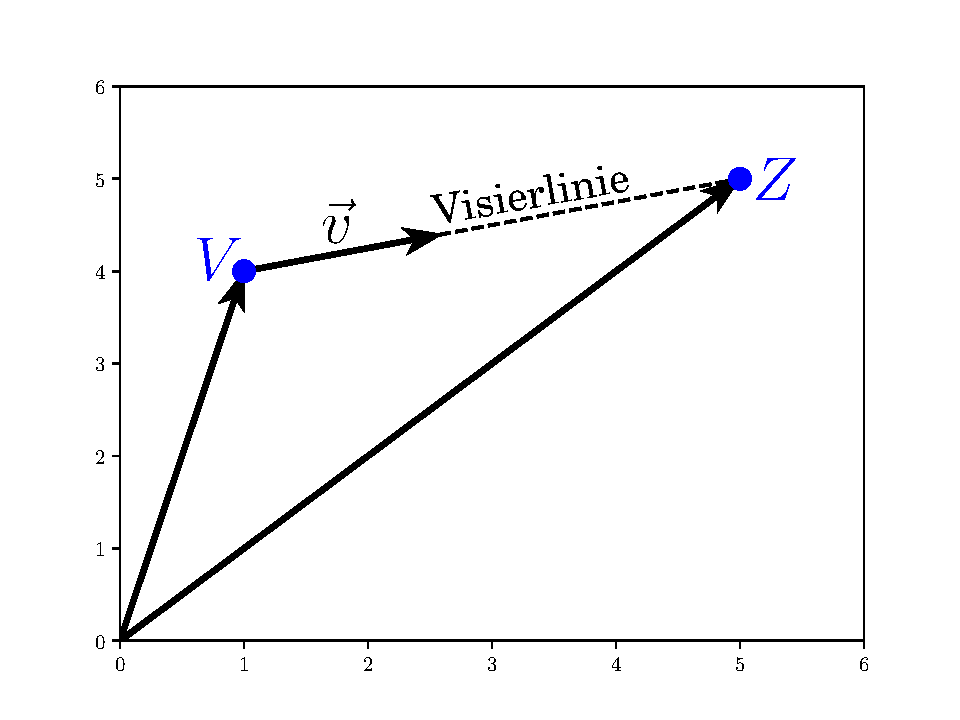
\includegraphics[scale=0.6]{./papers/lambertw/Bilder/Strategie.pdf}
    \caption{Vektordarstellung Jagdstrategie}
    \label{lambertw:grafic:pursuerDGL2}
\end{figure}
%
In der Tabelle \ref{lambertw:table:Strategien} sind drei mögliche Strategien aufgezählt.
Im Folgenden wird nur noch auf die Jagdstrategie eingegangen.
Bei dieser Strategie ist die Geschwindigkeit konstant und der Verfolger bewegt sich immer direkt auf sein Ziel zu.
Der Verfolger und sein Ziel werden als Punkte $V$ und $Z$ modelliert.
In der Abbildung \ref{lambertw:grafic:pursuerDGL2} ist das Problem dargestellt,
wobei $v$ der Ortsvektor des Verfolgers, $z$ der Ortsvektor des Ziels und $\dot{v}$ der Geschwindigkeitsvektor des Verfolgers ist.
Der Geschwindigkeitsvektor entspricht dem Richtungsvektors des Verfolgers.
Die konstante Geschwindigkeit kann man mit
%
\begin{equation}
    |\dot{v}|
    = \operatorname{const} = A
    \text{,}\quad A\in\mathbb{R}^+
\end{equation}
%
darstellen. Der Geschwindigkeitsvektor muss auf das Ziel zeigen, woraus folgt
\begin{equation}
    \dot{v}
    \quad||\quad
    z-v
    \text{.}
\end{equation}
Um den Richtungsvektor zu konstruieren kann der Einheitsvektor parallel zu $z-v$ um $|\dot{v}|$ gestreckt werden, was zu
\begin{equation}
    \dot{v}
    =
    |\dot{v}|\cdot (z-v)^\circ
    =
    |\dot{v}|\cdot\frac{z-v}{|z-v|}
    \label{lambertw:richtungsvektor}
\end{equation}
führt.
Aus dem Verfolgungsproblem ist auch ersichtlich, dass die Punkte $V$ und $Z$ nicht am gleichen Ort starten und so eine Division durch Null ausgeschlossen ist.
Wenn die Punkte $V$ und $Z$ trotzdem am gleichen Ort starten, ist die Lösung trivial.

Nun wird die Gleichung mit $\dot{v}$ skalar multipliziert, um das Gleichungssystem von zwei auf eine Gleichung zu reduzieren. Somit ergibt sich
\begin{align}
    \frac{z-v}{|z-v|}\cdot|\dot{v}|\cdot\dot{v}
    &=
    |\dot{v}|^2
    \text{,}
\end{align}
was algebraisch zu
\begin{align}
    \label{lambertw:pursuerDGL}
    \frac{z-v}{|z-v|}\cdot \frac{\dot{v}}{|\dot{v}|}
    &=
    1
\end{align}
umgeformt werden kann.
Die Lösungen dieser Differentialgleichung sind die gesuchten Verfolgungskurven, sofern der Verfolger die Jagdstrategie verwendet.
%
\subsection{Ziel
\label{lambertw:subsection:Ziel}}
Als nächstes gehen wir auf das Ziel ein.
Wie der Verfolger wird auch unser Ziel sich strikt an eine Fluchtstrategie halten, welche von Anfang an bekannt ist.
Als Strategie eignet sich eine definierte Fluchtkurve oder ähnlich wie beim Verfolger ein Verhalten, das vom Verfolger abhängig ist.
Ein vom Verfolger abhängiges Verhalten führt zu einem gekoppeltem DGL-System, das schwierig zu lösen sein wird.
Eine definierte Fluchtkurve kann mit einer Parameterdarstellung der Position nach der Zeit beschrieben werden.
Zum Beispiel könnte ein Ziel auf einer Geraden flüchten, welches auf einer Ebene mit der Parametrisierung
%
\begin{equation}
    z(t)
    =
    \left( \begin{array}{c} 0 \\  t \end{array} \right)
\end{equation}
%
beschrieben werden könnte.
Mit dieser Gleichung ist das Ziel auch schon vollumfänglich definiert.
Für die Fluchtkurve kann eine beliebige Form gewählt werden, jedoch wird die zu lösende Differentialgleichung für die Verfolgungskurve komplexer.




